\section{Results}
\label{sec:results}

\subsection{Main Experiment: Accuracy vs.\ Character Count}

\Tabref{tab:main_results} presents accuracy for the main experiment.
Both models achieve perfect or near-perfect accuracy up to 16~characters.
Degradation begins at 32~characters, where \gptmini maintains 95.9\% accuracy [95\% CI: 93.8\%, 97.8\%] while \gptfull drops to 86.9\% [83.1\%, 90.6\%].

\begin{table}[t]
\centering
\caption{Main experiment accuracy (\%) by character count. Both models are perfect through 16 characters. 95\% bootstrap CIs shown in brackets where accuracy is below 100\%. Best result per column in \textbf{bold}.}
\label{tab:main_results}
\small
\begin{tabular}{@{}lccccc@{}}
\toprule
\textbf{Model} & \textbf{2} & \textbf{4} & \textbf{8} & \textbf{16} & \textbf{32} \\
\midrule
\gptmini & 100.0 & 100.0 & 100.0 & {\bf 100.0} & {\bf 95.9}~{\scriptsize [93.8, 97.8]} \\
\gptfull & 100.0 & 100.0 & 100.0 & 99.4~{\scriptsize [98.1, 100]} & 86.9~{\scriptsize [83.1, 90.6]} \\
\midrule
\randombaseline & 9.7 & 7.3 & 6.1 & 5.9 & 5.7 \\
\initialstate & 29.4 & 28.8 & 28.6 & 28.5 & 28.4 \\
\bottomrule
\end{tabular}
\end{table}

\subsection{Extended Experiment: Scaling to 64 Characters}

\Figref{fig:degradation} shows the accuracy degradation curve from the extended experiment, which pushes to 64~characters.
\Tabref{tab:extended_results} gives the corresponding numbers.

\begin{figure}[t]
\centering
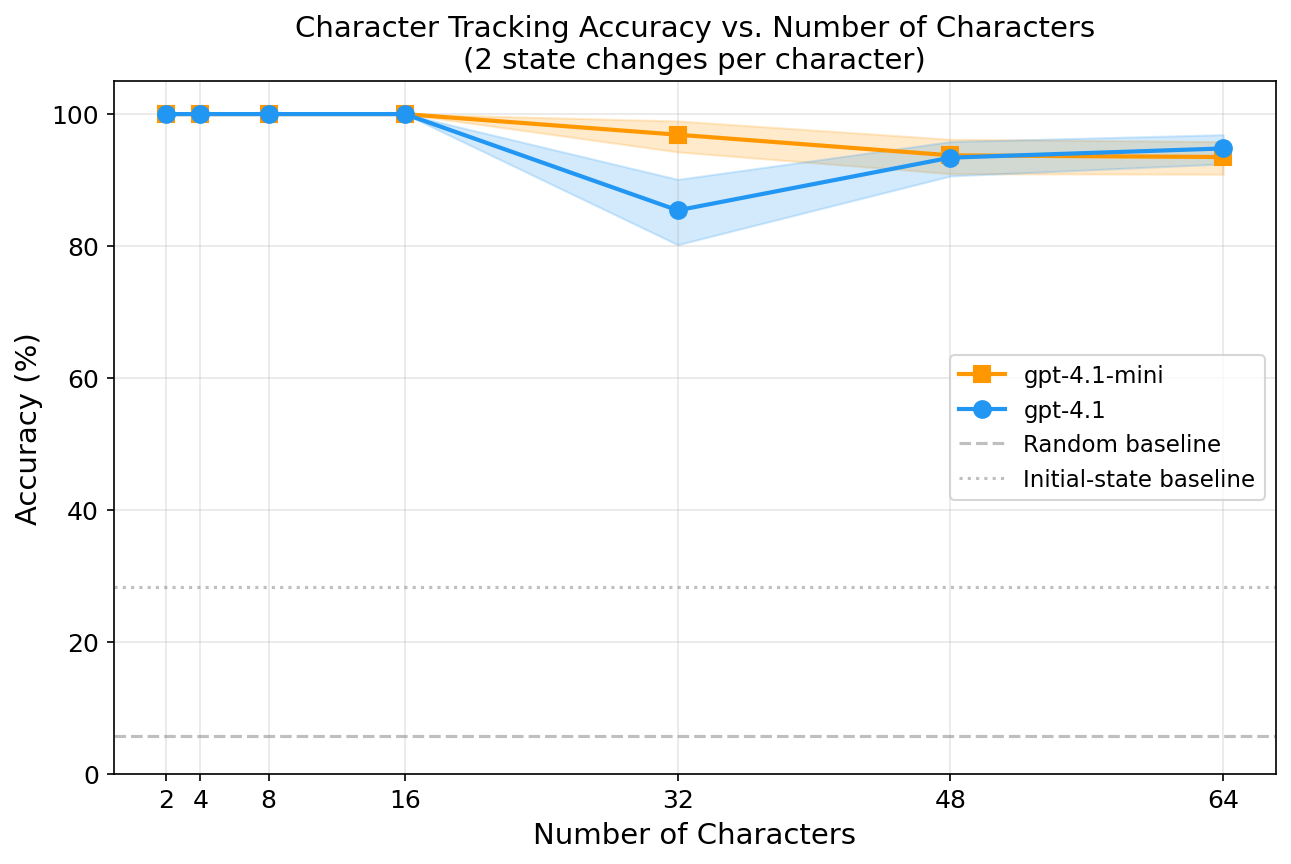
\includegraphics[width=0.95\linewidth]{figures/degradation_curve.png}
\caption{Accuracy vs.\ character count for both models (extended experiment). Shaded regions indicate 95\% bootstrap confidence intervals. Both models maintain $>$93\% accuracy through 64~characters, with no sharp cliff. \gptmini (blue) is consistently at or above \gptfull (orange) beyond 16~characters.}
\label{fig:degradation}
\end{figure}

\begin{table}[t]
\centering
\caption{Extended experiment accuracy (\%) across 2--64 characters. Best per column in \textbf{bold}.}
\label{tab:extended_results}
\small
\begin{tabular}{@{}lccccccc@{}}
\toprule
\textbf{Model} & \textbf{2} & \textbf{4} & \textbf{8} & \textbf{16} & \textbf{32} & \textbf{48} & \textbf{64} \\
\midrule
\gptmini & 100.0 & 100.0 & 100.0 & {\bf 100.0} & {\bf 96.9} & {\bf 93.8} & 93.5 \\
\gptfull & 100.0 & 100.0 & 100.0 & {\bf 100.0} & 85.4 & 93.4 & {\bf 94.8} \\
\bottomrule
\end{tabular}
\end{table}

Both models maintain above 93\% accuracy even at 64~characters.
Notably, \gptfull shows a non-monotonic pattern: accuracy dips at 32~characters (85.4\%) but recovers at 48 and 64 characters.
We discuss possible explanations in \secref{sec:discussion}.
\gptmini degrades monotonically and smoothly, consistent with a gradual capacity limit.

\subsection{Error Analysis}

\Figref{fig:error_types} shows the distribution of error types across character counts.
\Tabref{tab:errors} summarizes the aggregate error breakdown.

\begin{figure}[t]
\centering
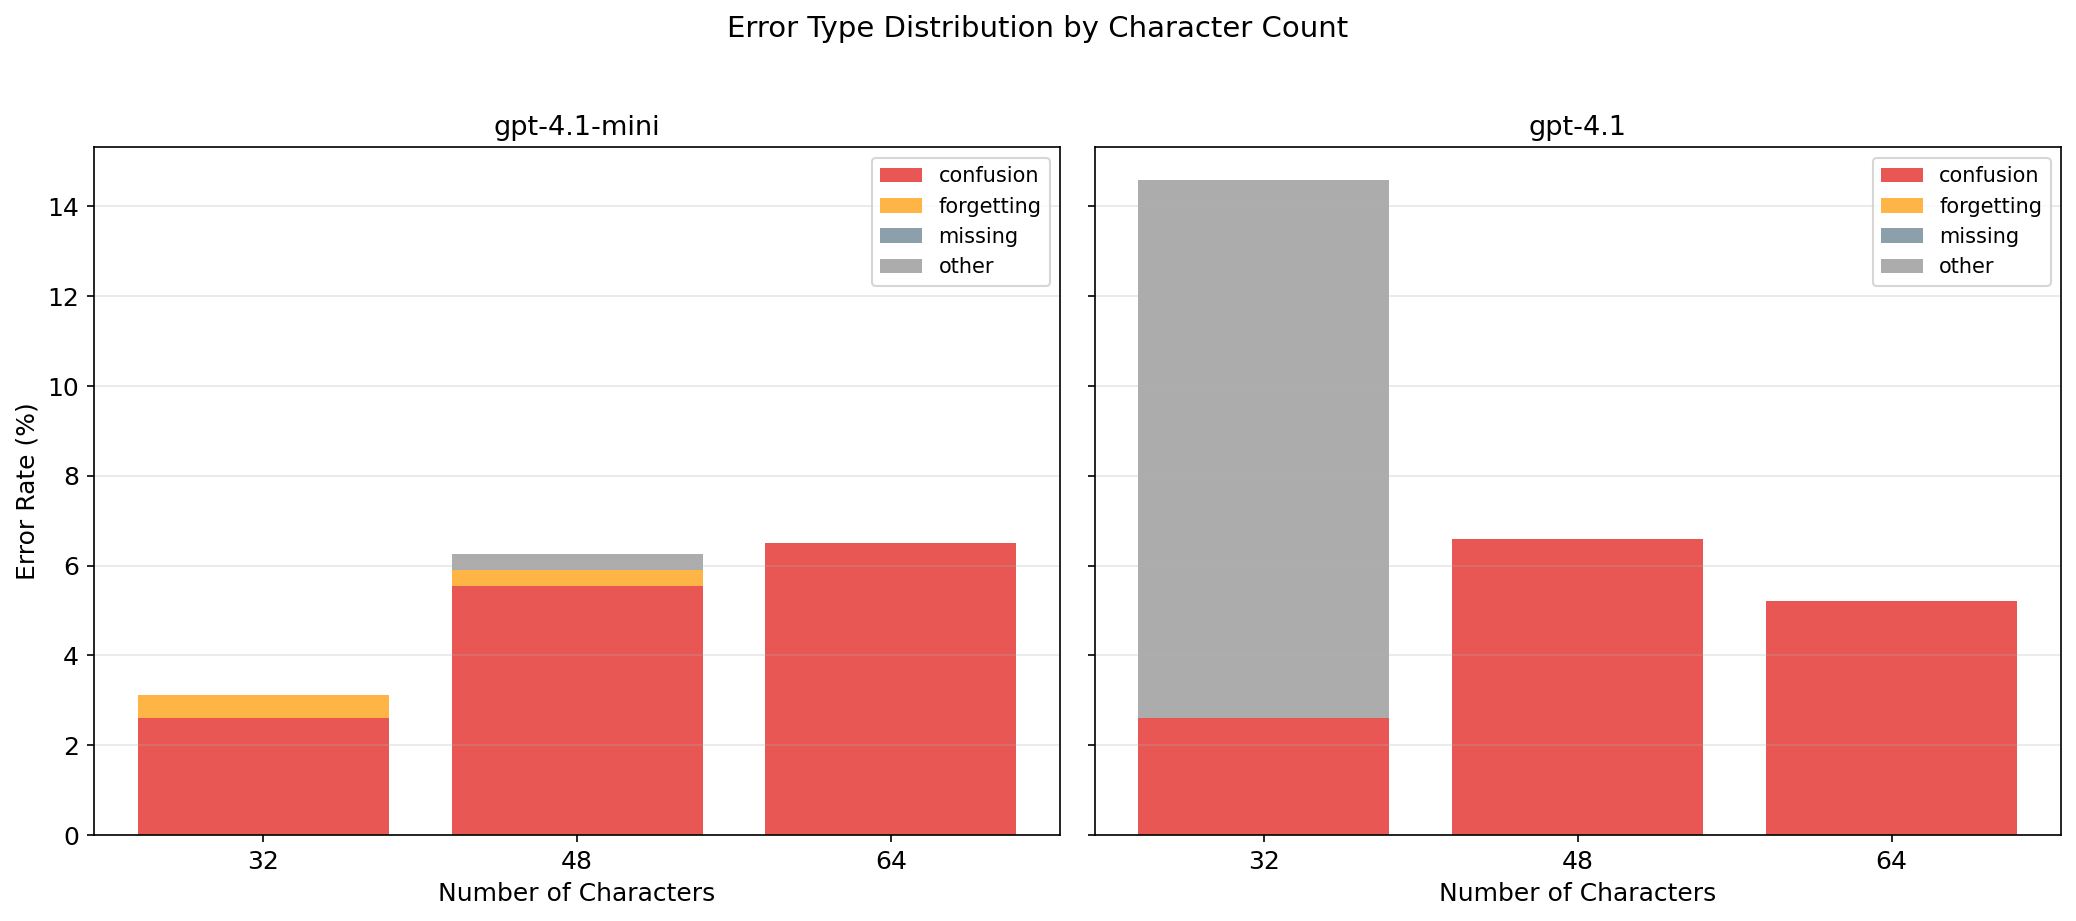
\includegraphics[width=0.95\linewidth]{figures/error_types.png}
\caption{Error type distribution by character count in the extended experiment. Confusion errors (swapping an attribute with another character's value) dominate for both models, especially for \gptmini where they account for 93.9\% of all errors.}
\label{fig:error_types}
\end{figure}

\begin{table}[t]
\centering
\caption{Error type distribution in the extended experiment. Confusion errors dominate for both models. \gptfull's ``other'' errors are predominantly the model returning ``none'' for possessions.}
\label{tab:errors}
\small
\begin{tabular}{@{}lcccc@{}}
\toprule
\textbf{Model} & \textbf{Confusion} & \textbf{Forgetting} & \textbf{Other} & \textbf{Total} \\
\midrule
\gptmini & 46 (93.9\%) & 2 (4.1\%) & 1 (2.0\%) & 49 \\
\gptfull & 44 (65.7\%) & 0 (0.0\%) & 23 (34.3\%) & 67 \\
\bottomrule
\end{tabular}
\end{table}

\para{Confusion errors dominate.}
For \gptmini, 93.9\% of all errors are confusions---the model's answer is the correct current value for a different character.
Forgetting errors (reverting to the initial state) account for only 4.1\%.
\gptfull shows a similar pattern (65.7\% confusion) but with a substantial fraction of ``other'' errors (34.3\%), which we analyze below.

\para{\gptfull's ``none'' errors.}
\gptfull's ``other'' errors at 32~characters are predominantly cases where the model returns ``none'' for a character's possession.
Inspection reveals that these occur on compound drop-then-pickup sentences (\eg ``Diana set down a crystal vial. Diana picked up a golden key'').
The model correctly processes the drop event but fails to register the subsequent pickup, suggesting an attention-allocation limitation in sequential event processing.

\subsection{Stress Test: Increased State Changes}

\Tabref{tab:stress} compares accuracy with 2 vs.\ 4 state changes per character.
\Figref{fig:stress} visualizes the comparison.

\begin{table}[t]
\centering
\caption{Stress test accuracy (\%) with 4 state changes per character, compared to the main experiment (2 changes). \gptmini is remarkably robust; \gptfull degrades substantially.}
\label{tab:stress}
\small
\begin{tabular}{@{}lcccc@{}}
\toprule
\textbf{Model} & \textbf{4 chars} & \textbf{8 chars} & \textbf{16 chars} & \textbf{32 chars} \\
\midrule
\gptmini (2 changes) & 100.0 & 100.0 & 100.0 & 95.9 \\
\gptmini (4 changes) & 100.0 & 97.9 & 97.9 & {\bf 97.4} \\
\midrule
\gptfull (2 changes) & 100.0 & 100.0 & 99.4 & 86.9 \\
\gptfull (4 changes) & 100.0 & 97.9 & 91.7 & 84.4 \\
\bottomrule
\end{tabular}
\end{table}

\begin{figure}[t]
\centering
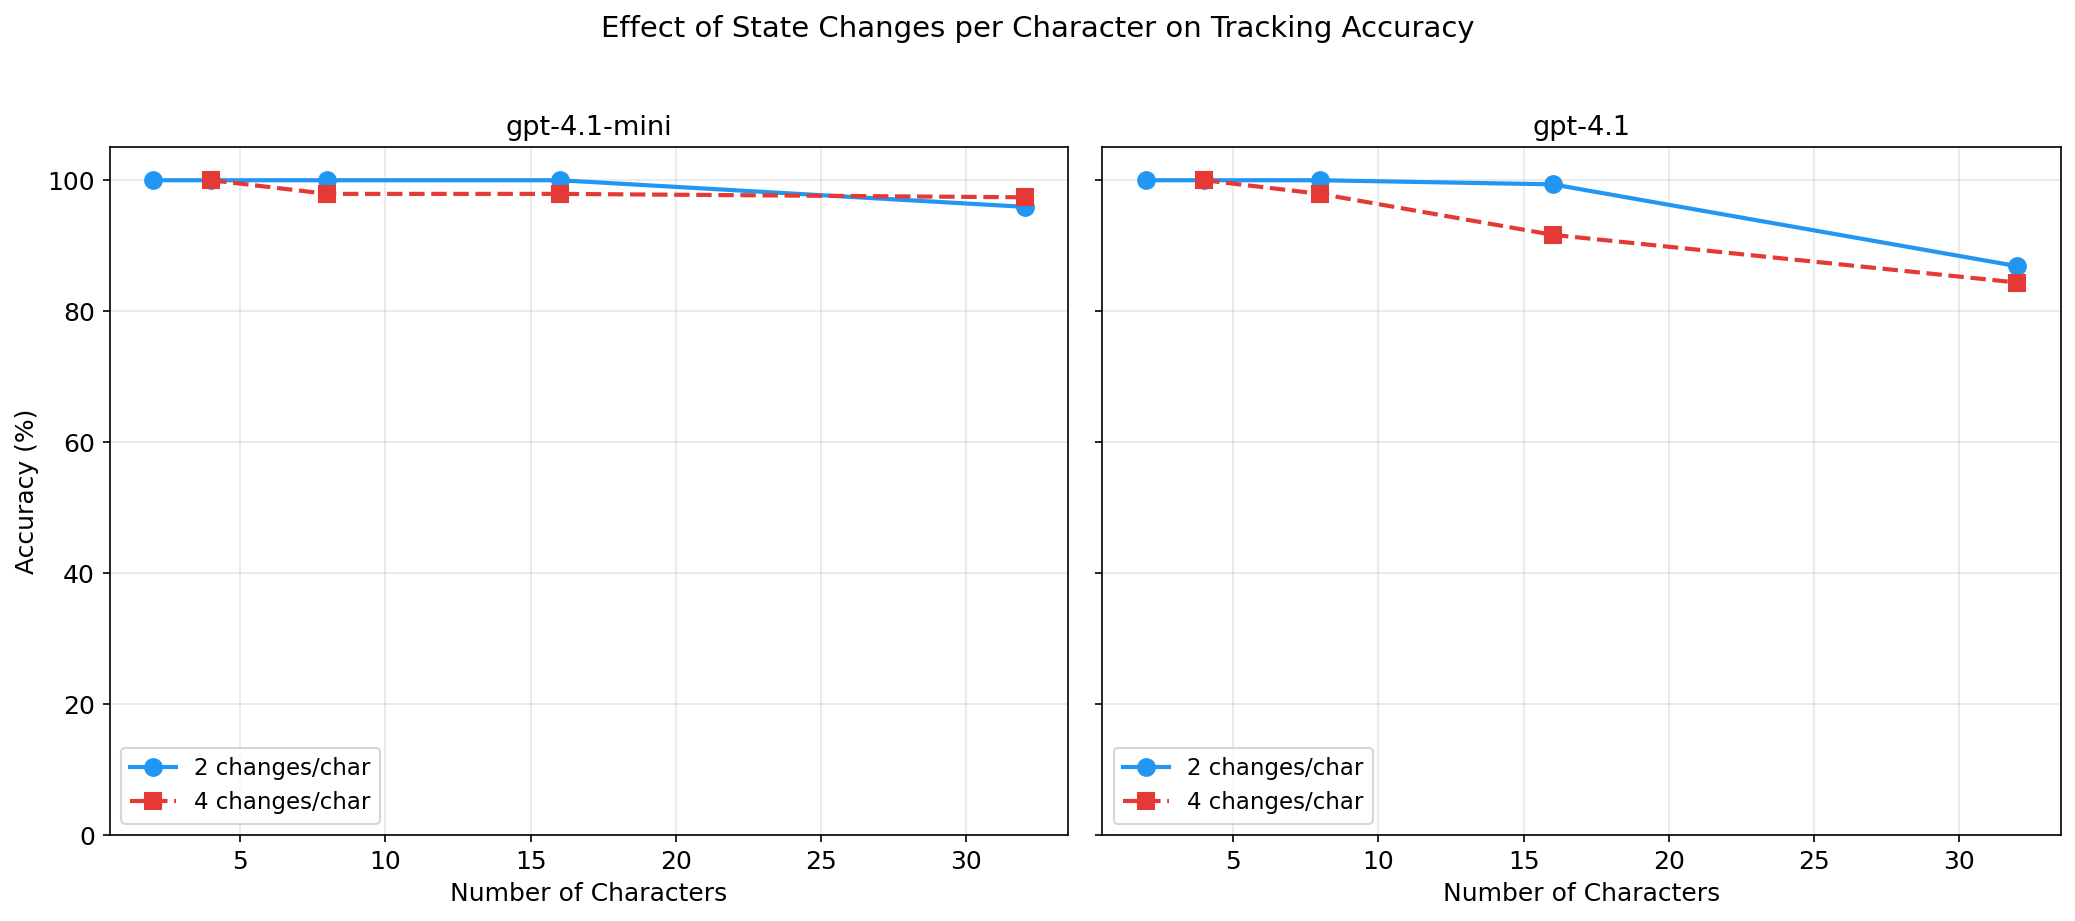
\includegraphics[width=0.95\linewidth]{figures/stress_comparison.png}
\caption{Accuracy comparison between 2 and 4 state changes per character. \gptmini is remarkably robust to increased state-change density, while \gptfull shows meaningful degradation at 16 and 32 characters.}
\label{fig:stress}
\end{figure}

Doubling state changes has a modest effect on \gptmini (97.4\% at 32~characters with 4 changes vs.\ 95.9\% with 2 changes) but a larger effect on \gptfull (84.4\% vs.\ 86.9\% at 32~characters, and 91.7\% vs.\ 99.4\% at 16~characters).

\subsection{Position and Attribute Effects}

\para{No lost-in-the-middle effect.}
Character introduction order does not significantly predict accuracy for \gptmini (Spearman $r = 0.024$, $p = 0.45$).
\gptfull shows a small but statistically significant effect ($r = 0.088$, $p = 0.006$), with later-introduced characters tracked slightly \emph{better}---the opposite of a primacy advantage.
Overall, the ``lost in the middle'' effect~\citep{liu2024lost} does not manifest strongly in our setting.

\para{Location vs.\ possession tracking.}
\Figref{fig:attribute} compares accuracy on location and possession queries.
Both attribute types show similar degradation patterns, with one notable exception: \gptfull at 32~characters achieves 99.0\% on location queries but only 71.9\% on possession queries.
This asymmetry is driven by the compound drop-then-pickup failure mode described above.

\begin{figure}[t]
\centering
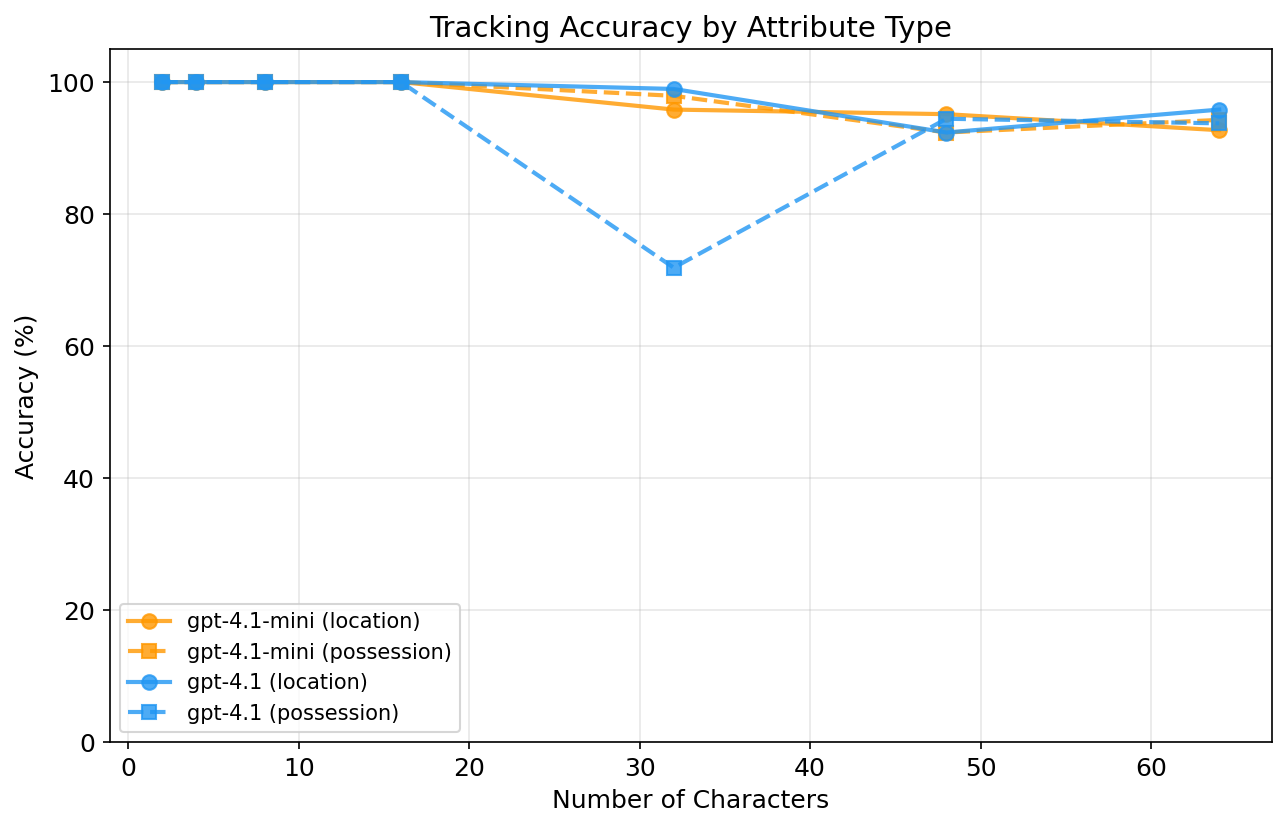
\includegraphics[width=0.95\linewidth]{figures/attribute_comparison.png}
\caption{Accuracy by attribute type (location vs.\ possession). The two attribute types degrade similarly, except for \gptfull at 32~characters, where possession tracking drops sharply due to compound-sentence parsing failures.}
\label{fig:attribute}
\end{figure}

\subsection{Statistical Significance}

\Tabref{tab:stats} reports Spearman correlations between character count and accuracy.
\gptmini shows a small but significant negative correlation ($r = -0.104$, $p = 0.0007$), confirming that accuracy degrades with character count.
\gptfull's correlation is not significant ($r = 0.005$, $p = 0.86$) due to its non-monotonic accuracy pattern.

\begin{table}[t]
\centering
\caption{Spearman rank correlations. The character-count effect is significant for \gptmini but not \gptfull (due to non-monotonicity). Neither model shows a strong position effect.}
\label{tab:stats}
\small
\begin{tabular}{@{}llcc@{}}
\toprule
\textbf{Test} & \textbf{Model} & \textbf{$r$} & \textbf{$p$} \\
\midrule
Char count vs.\ accuracy & \gptmini & $-0.104$ & 0.0007 \\
Char count vs.\ accuracy & \gptfull & $0.005$ & 0.86 \\
Position vs.\ accuracy & \gptmini & $0.024$ & 0.45 \\
Position vs.\ accuracy & \gptfull & $0.088$ & 0.006 \\
\bottomrule
\end{tabular}
\end{table}
